\section{Mesures intermédiaires sur le capteur}
\label{chap:mesures}
\subsection{Vérification du corps de chauffe}
Avant toute chose, afin de pouvoir suivre tous les paramètres et le fonctionnement du capteur \gls{capteur}, une caméra thermique a été utilisée
pour observer le comportement du corps de chauffe.

\begin{figure}[H]
    \hspace{-0.3 cm}
    \begin{subfigure}{0.3\textwidth}
        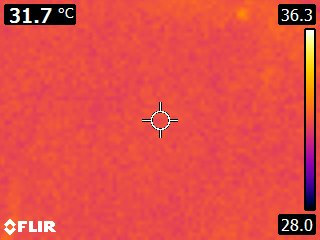
\includegraphics[scale = 0.45]{assets/figures/thermique_sans_chauffe.jpg}
        \caption{Image thermique du capteur - Corps de chauffe éteint}
    \end{subfigure}
    \hspace{0.2cm}
    \begin{subfigure}{0.3\textwidth}
        \centering
        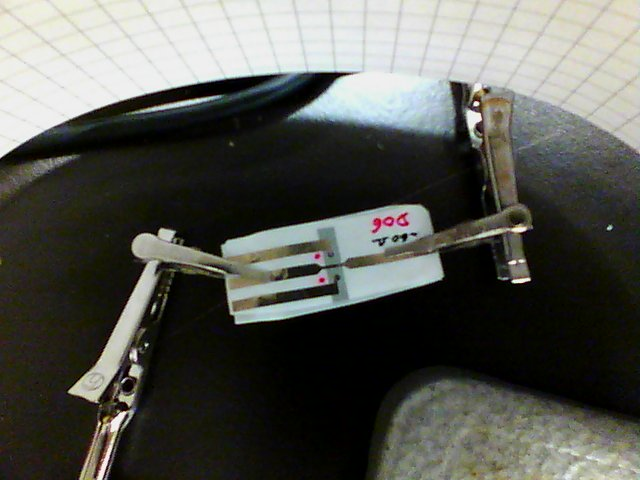
\includegraphics[scale = 0.23]{assets/figures/visuel_avec_chauffe.jpg}
        \caption{Image numérique}
    \end{subfigure}
    \hspace{0.5cm}
    \begin{subfigure}{0.3\textwidth}
        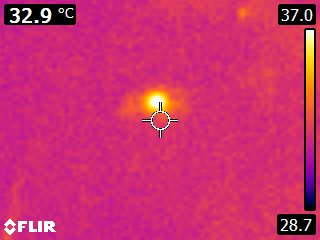
\includegraphics[scale = 0.5]{assets/figures/thermique_avec_chauffe.jpg}
        \caption{Image thermique du capteur - Corps de chauffe allumé}
    \end{subfigure}
    \caption{D06 - Résultats de la caméra thermique}
    \label{fig:cameraThermique}
\end{figure}

Il faut savoir que les pistes d'or réfléchissent énormément. Il est donc difficile d'obtenir un résultat parfait. Une première astuce a été de
dessiner au stylo un point noir sur les pistes à mesurer. Ainsi, les problèmes de réflexions seraient amoindris. Malheureusement cette astuce n'a
pas été suffisante. \\

Une autre mesure a alors été faite dans des conditions moins lumineuses (après le coucher du soleil). La figure \ref*{fig:cameraThermique},
montre que le corps de chauffe de l'échantillon D06 possède une température avoisinant les 37\textdegree C lorsqu'un courant de 15 mA y circule. \\

Les tests de chauffe à la caméra ont été effectué sur d'autres échantillons tels que les échantillons D12, D13 et D14. Malheureusement ces derniers 
n'ont donné aucun résultat à la caméra thermique (aucun signe d'échauffement). Le corps de chauffe devra donc être amélioré en épaississant la 
couche d'or formé par la \gls{pvd} et/ou en modifiant la forme générale du corps de chauffe. 

\subsection{Vérification des résistances}
Un second type de mesure permettant de comprendre chaque partie du \gls{capteur} a été effectuée. Celle-ci concerne la résistance du corps de
chauffe et du circuit thermoélectrique.

\begin{table}[H]
    \begin{center}
        \begin{tabular}{|p{2cm}|p{2cm}|p{1.7cm}|p{2.1cm}|p{2.1cm}|p{2.1cm}|p{2.1cm}|}
            \hline
                                 &                    &                  & \multicolumn{2}{|c|}{\textbf{Corps de chauffe}} & \multicolumn{2}{|c|}{\textbf{Circuit du thermocouple}}                                                                                            \\
            \hline
            \textbf{Échantillon} & \textbf{Membranes} & \textbf{Méthode} & \textbf{Résistance directe} [$\Omega$]          & \textbf{Résistance pointes ressorts} [$\Omega$]        & \textbf{Résistance directe} [$\Omega$] & \textbf{Résistance pointes ressorts [$\Omega$]} \\
            \hline
            D06                  & GTTP               & A                & 74.29                                           & 75.3                                                   & 151.5                                  & 157                                             \\
            \hline
            D11                  & PI25005            & A                & 2.8                                             & 2.7                                                    & 35 000 000                             & 20 000 000                                      \\
            \hline
            D12                  & PI25005            & A                & 2.44                                            & 2.45                                                   & 5600                                   & 5580                                            \\
            \hline
            D13                  & PI25005            & B                & 6.07                                            & 6.14                                                   & 585.5                                  & 570.2                                           \\
            \hline
            D14                  & VCTP               & A                & 2.53                                            & 2.58                                                   & 6.83                                   & 6.91                                            \\
            \hline
        \end{tabular}
        \caption{Résistances sur le capteur}
        \label{tab:resistancePointeRessort}
    \end{center}
\end{table}

Sur le tableau \ref{tab:resistancePointeRessort}, une légère différence entre la résistance mesurée directement sur la piste d'or (résistance 
appelée Résistance directe) et la résistance à travers les pointes ressort est visible. Ceci peut être dû au fait que les pointes ressort ont 
également une petite résistance qui vient alors changer la résistance totale du corps de chauffe. Cependant, il faut également prendre en 
compte le fait que la résistance change suivant la position de la mesure. En effet, une mesure faite aux extrémités de la piste d'or sera différente 
d'une mesure effectuée sur le centre de la piste d'or. \\

L'échantillon D11 possède une résistance de thermocouple très instable et élevée. Pour cette raison, il a été décidé que, sur ce capteur, les 
mesures suivantes ne seront pas effectuées, car cet échantillon a peu de chance de donner des résultats concluants. 

\begin{comment}
\section{Résultats concluants}
Avec une nouvelle solution de Tellure de Bismuth et deux nouvelles électrodépositions sur une membrane de GTTP, de nouvelles mesures ont été
effectuées. Ces mesures nous ont montré que le capteur fonctionnait. En effet, une réponse a été mesurée.
\begin{table}[H]
    \begin{center}
        \begin{tabular}{|c|c|}
            \hline
            Condition du capteur                                   & Tension mesurée à travers l'amplificateur \\
            \hline
            Corps de chauffe désactivé et arrivée d'air désactivée & 5 mV                                      \\
            \hline
            Corps de chauffe activé et arrivée d'air désactivée    & 0 V                                       \\
            \hline
            Corps de chauffe activé et arrivée d'air activée       & 8 mV                                      \\
            \hline
        \end{tabular}
    \end{center}
\end{table}
Malgré le bruit non-négligeable mesuré à travers l'amplificateur, la tension change suivant les conditions du capteur. Afin de se concentrer
uniquement sur la réponse du capteur, l'amplificateur a été mis de côté pour les futures mesures.
\end{comment}

\section{Procédure de mesures "classiques"}
\begin{enumerate}
    \item Mesures avec un corps de chauffe pulsé\\
    \item Mesures avec un corps de chauffe pulsé et un flux d'air comprimé constant\\
    \item Mesures avec un flux d'air comprimé pulsé\\
    \item Mesures avec un flux d'air comprimé pulsé et un corps de chauffe constant\\
    \item Mesures sans corps de chauffe et une respiration humaine\\
    \item Mesures avec corps de chauffe constant et respiration humaine
\end{enumerate}
Ces mesures ont été effectuées sur les quatre échantillons décrits sur le tableau \ref{tab:resistancePointeRessort}. \\

Malheureusement, le problème du bruit conséquent sortant de l'amplificateur n'a pas pu être résolu pour ce projet. Toutes les mesures ont alors 
été effectuées directement sur le capteur \gls{capteur}, sans passer par l'amplificateur. 

\section{Mesures du capteur sans amplificateur}
Plusieurs mesures ont été faites avec plusieurs types de paramètres. Toutes les mesures avec leurs paramètres ont été regroupées et sauvegardées
dans un document Excel qui se trouve en annexe.\\
Chacune des mesures sur cet Excel est liée à un autre fichier contenant toutes les valeurs concernant cette mesure.
\begin{figure}[H]
    \centering
    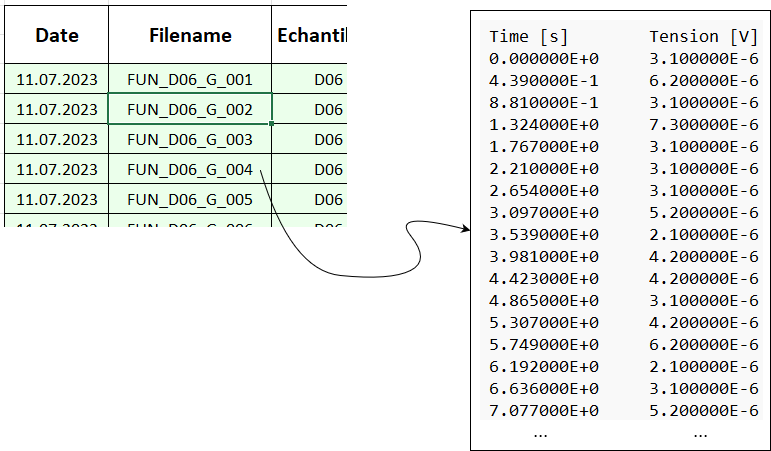
\includegraphics[scale = 0.4]{assets/figures/Data.png}
    \caption{Organisation des données}
    \label{fig:data_orga}
\end{figure}

Les mesures les plus significatives seront présentées dans ce rapport. \\

\subsection{Résultats avec utilisation du corps de chauffe}
\subsubsection{Corps de chauffe pulsé}
Des premières mesures ont été effectuées sans flux d'air. En effet, il est déjà intéressant d'observer le comportement du capteur
lorsque seulement le corps de chauffe est activé. Ce dernier est alimenté avec 15 mA. Les résultats sont les suivants :
\begin{figure}[H]
    \hspace{-0.5cm}
    \begin{subfigure}[b]{0.45\textwidth}
        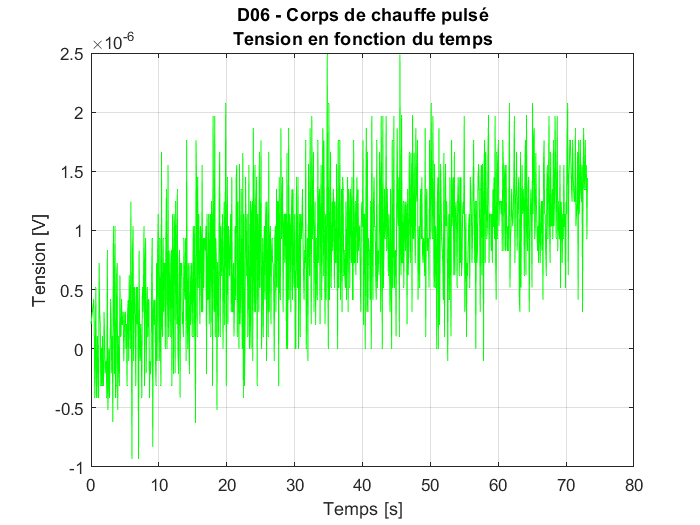
\includegraphics[scale = 0.45]{assets/figures/D06_corps_chauffe_pulse_green.png}
        \caption{Support solution 5 - Corps de chauffe pulsé}
        \label{fig:chauffe_pulse_g}
    \end{subfigure}
    \begin{subfigure}[b]{0.45\textwidth}
        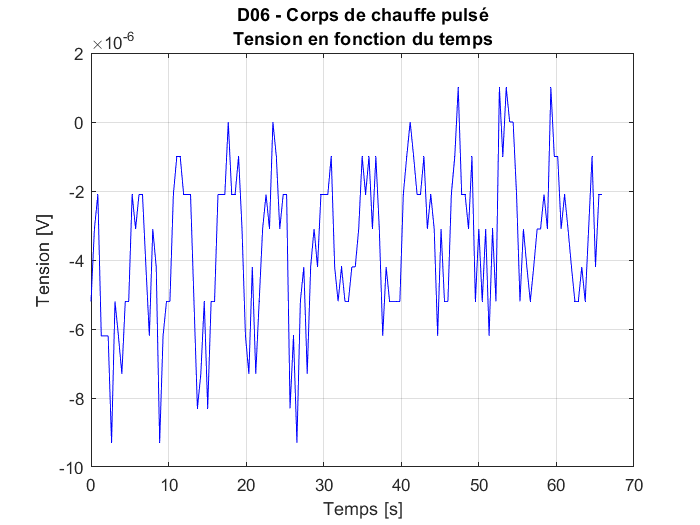
\includegraphics[scale = 0.45]{assets/figures/D06_corps_chauffe_pulse_blue.png}
        \caption{Support solution 1 - Corps de chauffe pulsé}
        \label{fig:chauffe_pulse_b}
    \end{subfigure}
\end{figure}

Sur la figure \ref{fig:chauffe_pulse_g}, aucun signal n'est distinguable. En effet, il semble n'y avoir que du bruit. \\

Cependant, sur la figure \ref{fig:chauffe_pulse_b}, la tension forme un certain signal. Pourtant, aucun flux n'est encore ajouté. \\
La raison de ce phénomène peut se trouver dans le fait que chaque électrodéposition est faite à la main, une après l'autre. Ceci signifie que
les deux électrodépositions diffèrent certainement l'une de l'autre. \\
De plus, le corps de chauffe est assez proche des deux électrodépositions. De ce fait, il est probable que lorsqu'il est en marche, le corps de
chauffe transfert de la chaleur aux deux extrémités en "L" du capteur. Ces deux extrémités sont alors chauffées, mais comme elles possèdent des nanofils
quelque peu différents d'un côté ou de l'autre, un gradient de température se forme et une certaine tension circule. \\
C'est une hypothèse du phénomène que l'on peut observer sur la figure \ref{fig:chauffe_pulse_b}.\\

Le support solution 5 semble, lui, éviter ce transfert de chaleur. Cela peut être dû au fait qu'étant donné que la membrane est plaquée contre
la base du support, la chaleur transférée par le corps de chauffe est "perdue" dans la matière du support (ici : PLA).\\

Pour ces raisons, le support solution 1 a été privilégié étant donné qu'il semble plus sensible que le support solution 5.\\

\subsubsection{Corps de chauffe constant et flux d'air comprimé pulsé}
La figure \ref{fig:test_cdc}, montre la réponse du capteur lorsqu'un flux d'air comprimé vient souffler sur le capteur pendant 3 s, puis 
stoppe le flux d'air pendant également 3 s. Après environ 50 s, le corps de chauffe est activé. 
\begin{figure}[H]
    \hspace{-0.3cm}
    \begin{subfigure}{0.45\textwidth}
        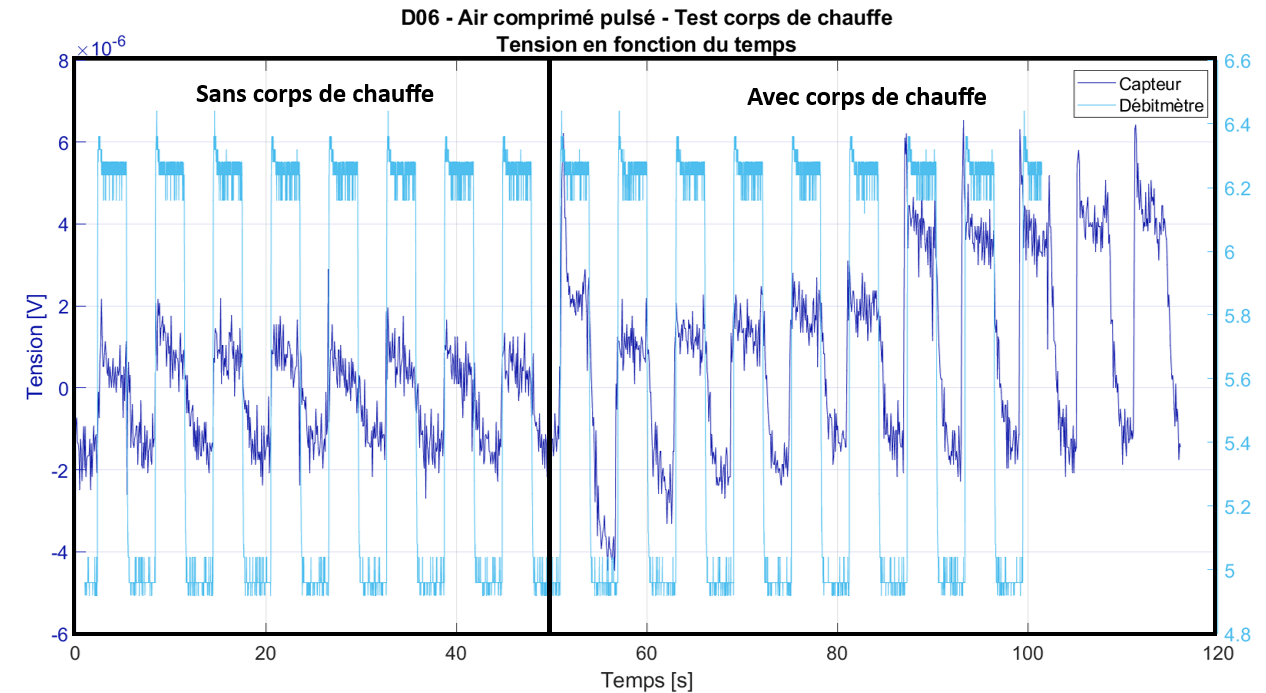
\includegraphics[scale = 0.4]{assets/figures/D06_air_pulse_test_cdc.png}
        \caption{D06 - Air comprimé pulsé - Sans, puis avec corps de chauffe}
        \label{fig:d06_test_cdc}
    \end{subfigure}
    \hspace{0.5cm}
    \begin{subfigure}{0.45\textwidth}
        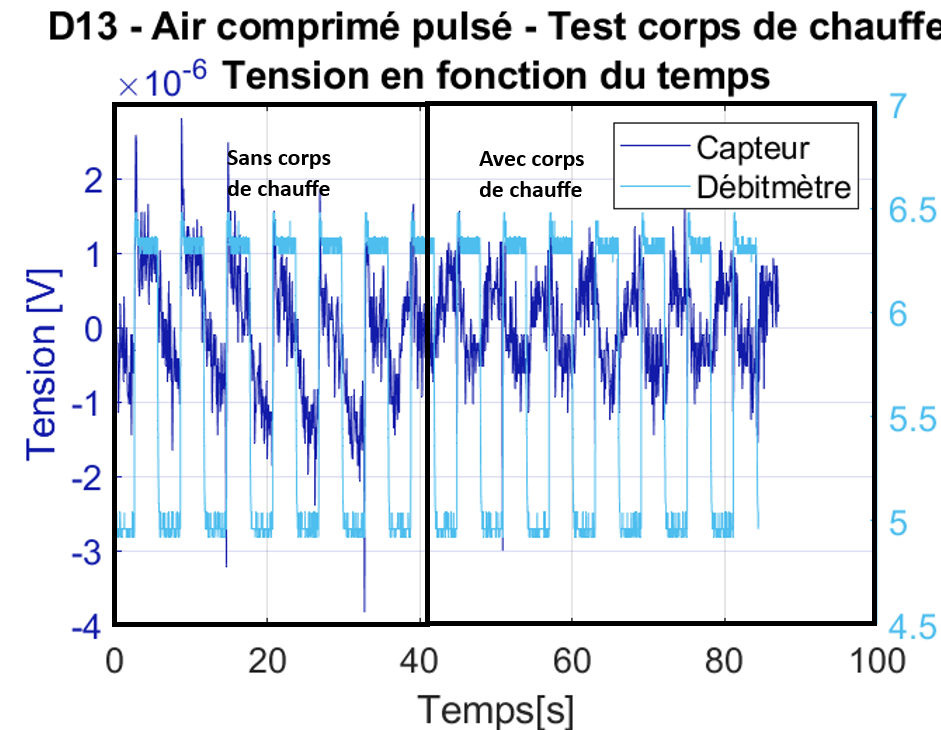
\includegraphics[scale = 0.4]{assets/figures/D13_air_comprime_pulse_test_cdc.png}
        \caption{D13 - Air comprimé pulsé - Sans, puis avec corps de chauffe}
        \label{fig:d13_test_cdc}
    \end{subfigure}
    \caption{Test corps de chauffe avec air comprimé pulsé}
    \label{fig:test_cdc}
\end{figure}

La figure \ref{fig:d06_test_cdc} nous permet de voir que le corps de chauffe a une influence sur la réponse du capteur. \\
Comme attendu, la figure \ref{fig:d13_test_cdc} représentant l'échantillon D13, ne montre pas une différence frappante avec ou sans corps de 
chauffe. Ce résultat était plutôt prévisible étant donné que les mesures à la caméra thermique ne donnait pas non plus de résultat pour cet 
échantillon. \\

Les différents résultats communiqués par les graphes soulignent que le corps de chauffe pourrait être amélioré. En effet, il serait intéressant 
à l'avenir de développer la géométrie générale du corps de chauffe. Par exemple, ce dernier pourrait être une piste d'or en configuration 
"serpentin". Ceci permettrait d'avoir un échauffement plus élevé. \\
Une autre solution serait d'épaissir la couche d'or. Elle serait peut-être moins fragile et il serait alors possible d'y amener un courant plus élevé. \\

Pour la suite des mesures, étant donné que le corps de chauffe n'offre pas un avantage notable, le corps de chauffe a été mis de côté. 

\begin{comment}
Par la suite, le sens par lequel est insufflé l'air a été testé. 
\begin{figure}[H]
    \centering
    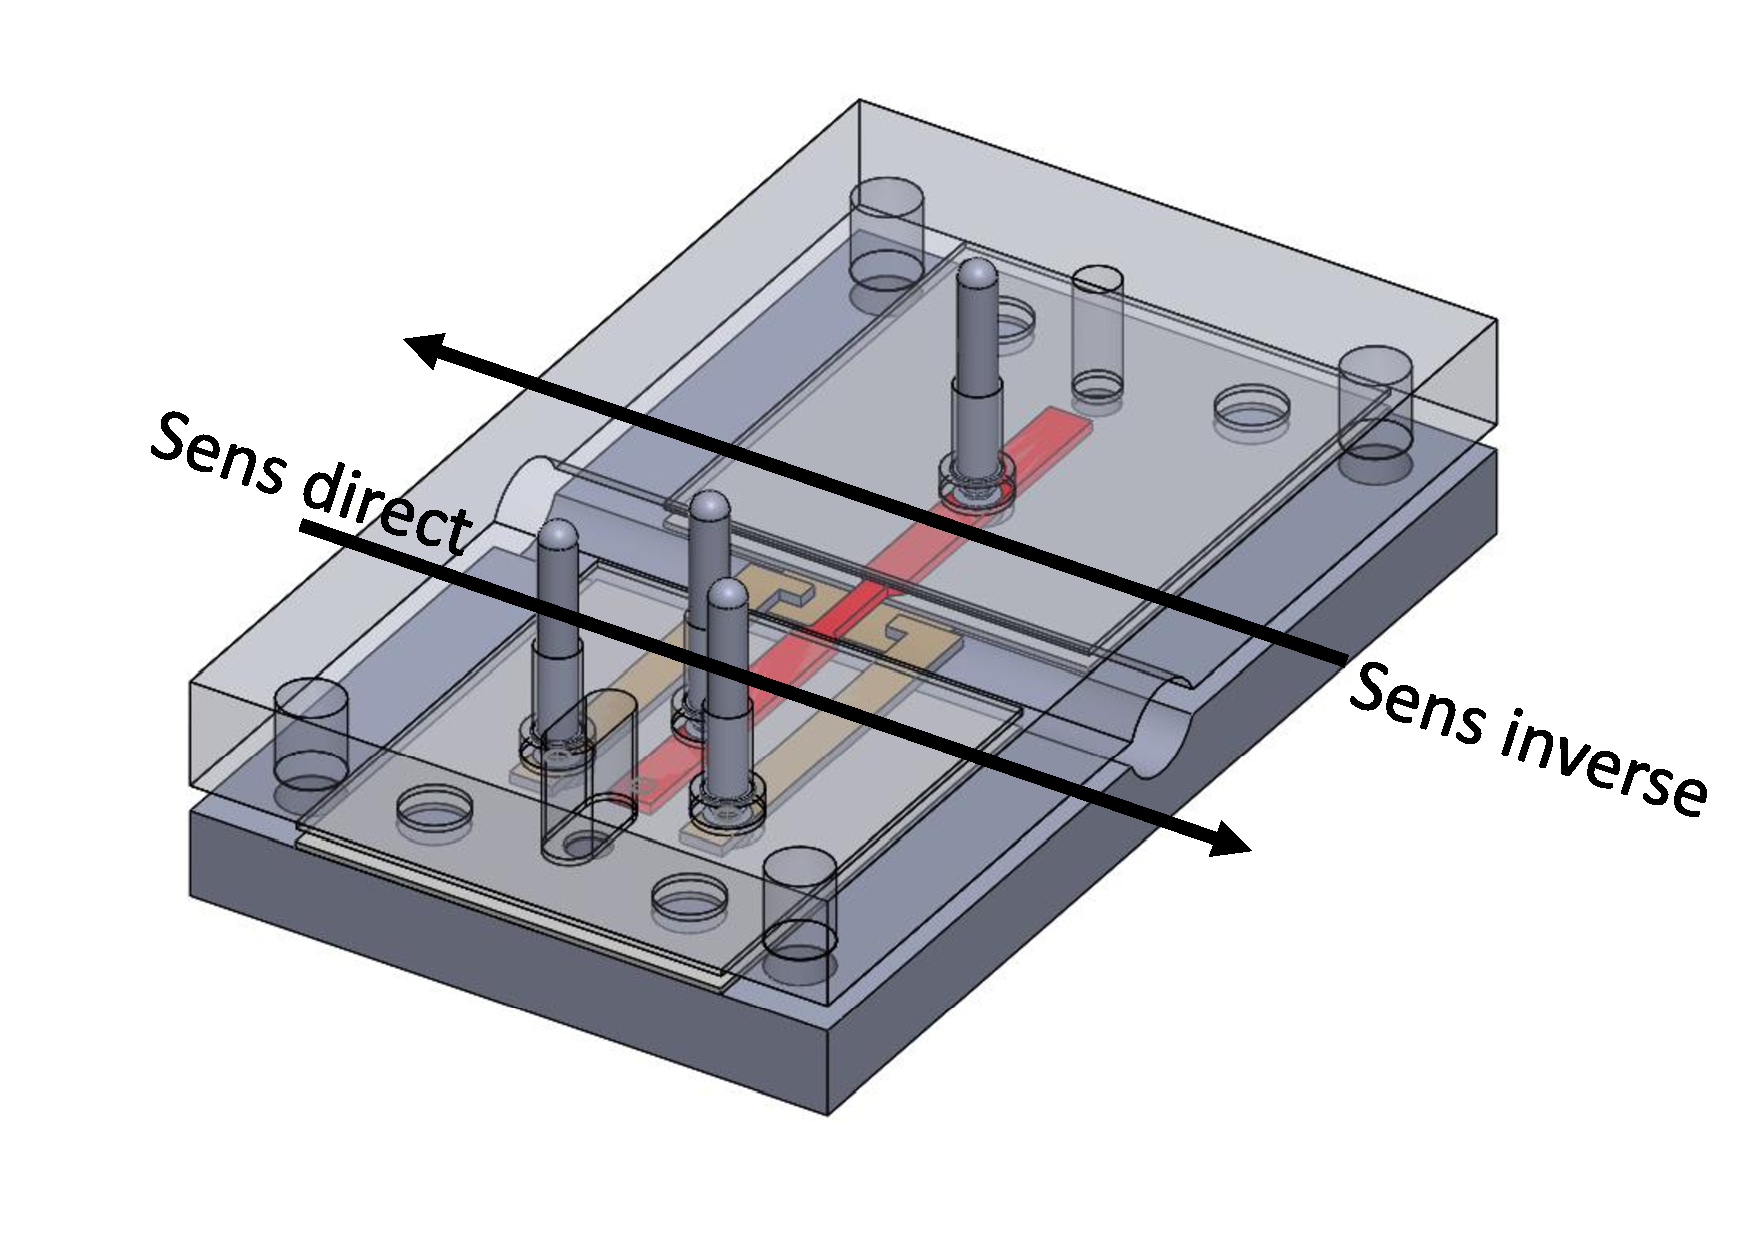
\includegraphics[scale = 0.3]{assets/figures/Inverse_direct.pdf}
    \caption{Sens direct ou inverse du flux d'air}
    \label{fig:direct_inverse}
\end{figure}

Sur la figure \ref{fig:D13_air_comp_pulse}, après environ 50 s, le tube d'arrivée d'air est débranché pour venir se rebrancher dans l'autre sens du capteur (sens direct vs sens inverse). 
Cette manipulation permet d'observer si un comportement différent est à noter. 

\begin{figure}[H]
    \centering
    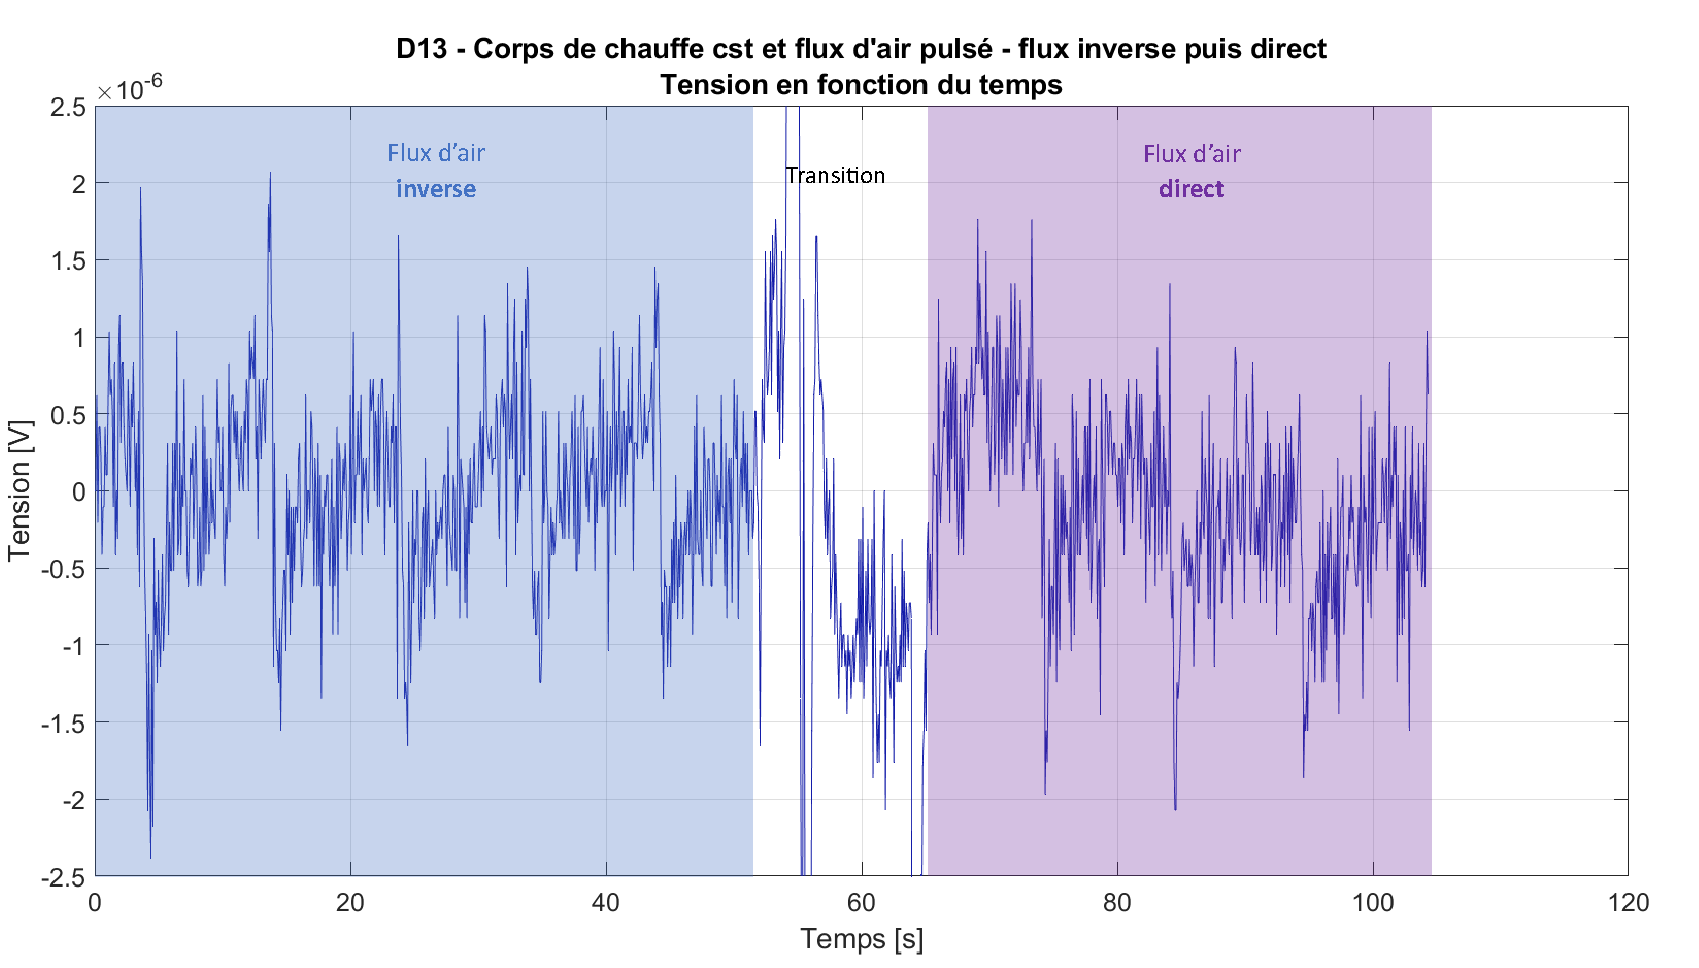
\includegraphics[scale = 0.6]{assets/figures/D13_air_comprime_pulse_blue.pdf}
    \caption{Échantillon D13 - Flux d'air comprimé pulsé en sens inverse puis direct}
    \label{fig:D13_air_comp_pulse}
\end{figure}
\end{comment}


\subsection{Respiration humaine}
Au lieu d'amener le flux d'air par une source d'air comprimé, l'arrivée d'air sera effectué par une respiration humaine. Ceci nous a donné les résultats suivants :

\begin{figure}[H]
    \hspace{-0.5cm}
    \begin{subfigure}{0.45\textwidth}
        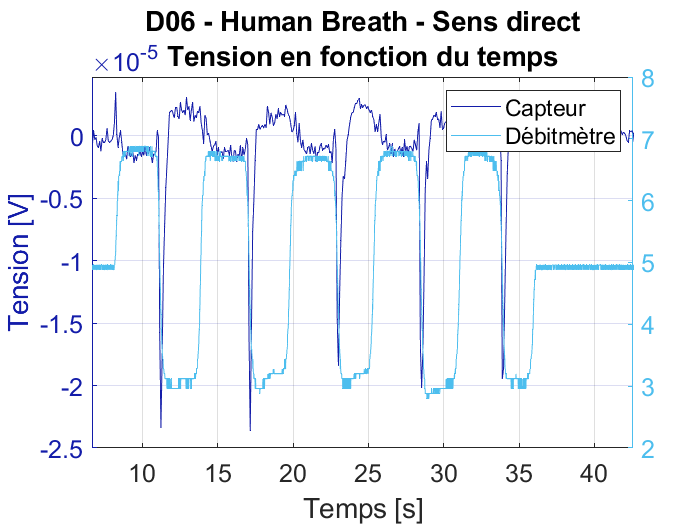
\includegraphics[scale = 0.45]{assets/figures/D06_hb_direct.png}
        \caption{D06 - Respiration humaine - Sens direct}
        \label{fig:d06_hb_direct}
    \end{subfigure}
    \hspace{0.7cm}
    \begin{subfigure}{0.45\textwidth}
        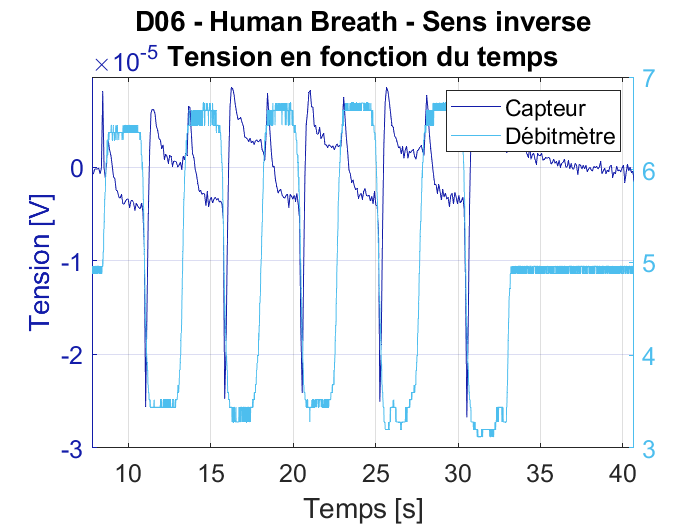
\includegraphics[scale = 0.45]{assets/figures/D06_hb_indirect.png}
        \caption{D06 - Respiration humaine - Sens indirect}
        \label{fig:d06_hb_indirect}
    \end{subfigure}
    \caption{D06 - Respiration humaine - Étude du sens direct et indirect}
\end{figure}
Ces figures permettent de construire une courbe tendance de la réponse du capteur \gls{capteur} en sens direct et inverse. C'est ce que représente 
la figure suivante :\\

////////////////////////iPad\\

Les graphes obtenus pour cet échantillon sont intéressants, car ils permettent d'observer plusieurs phénomènes. \\
\begin{enumerate}
    \item Un premier petit pic aparraît au début de l'expiration
    \item Un
\end{enumerate}

\begin{figure}[H]
    \centering
    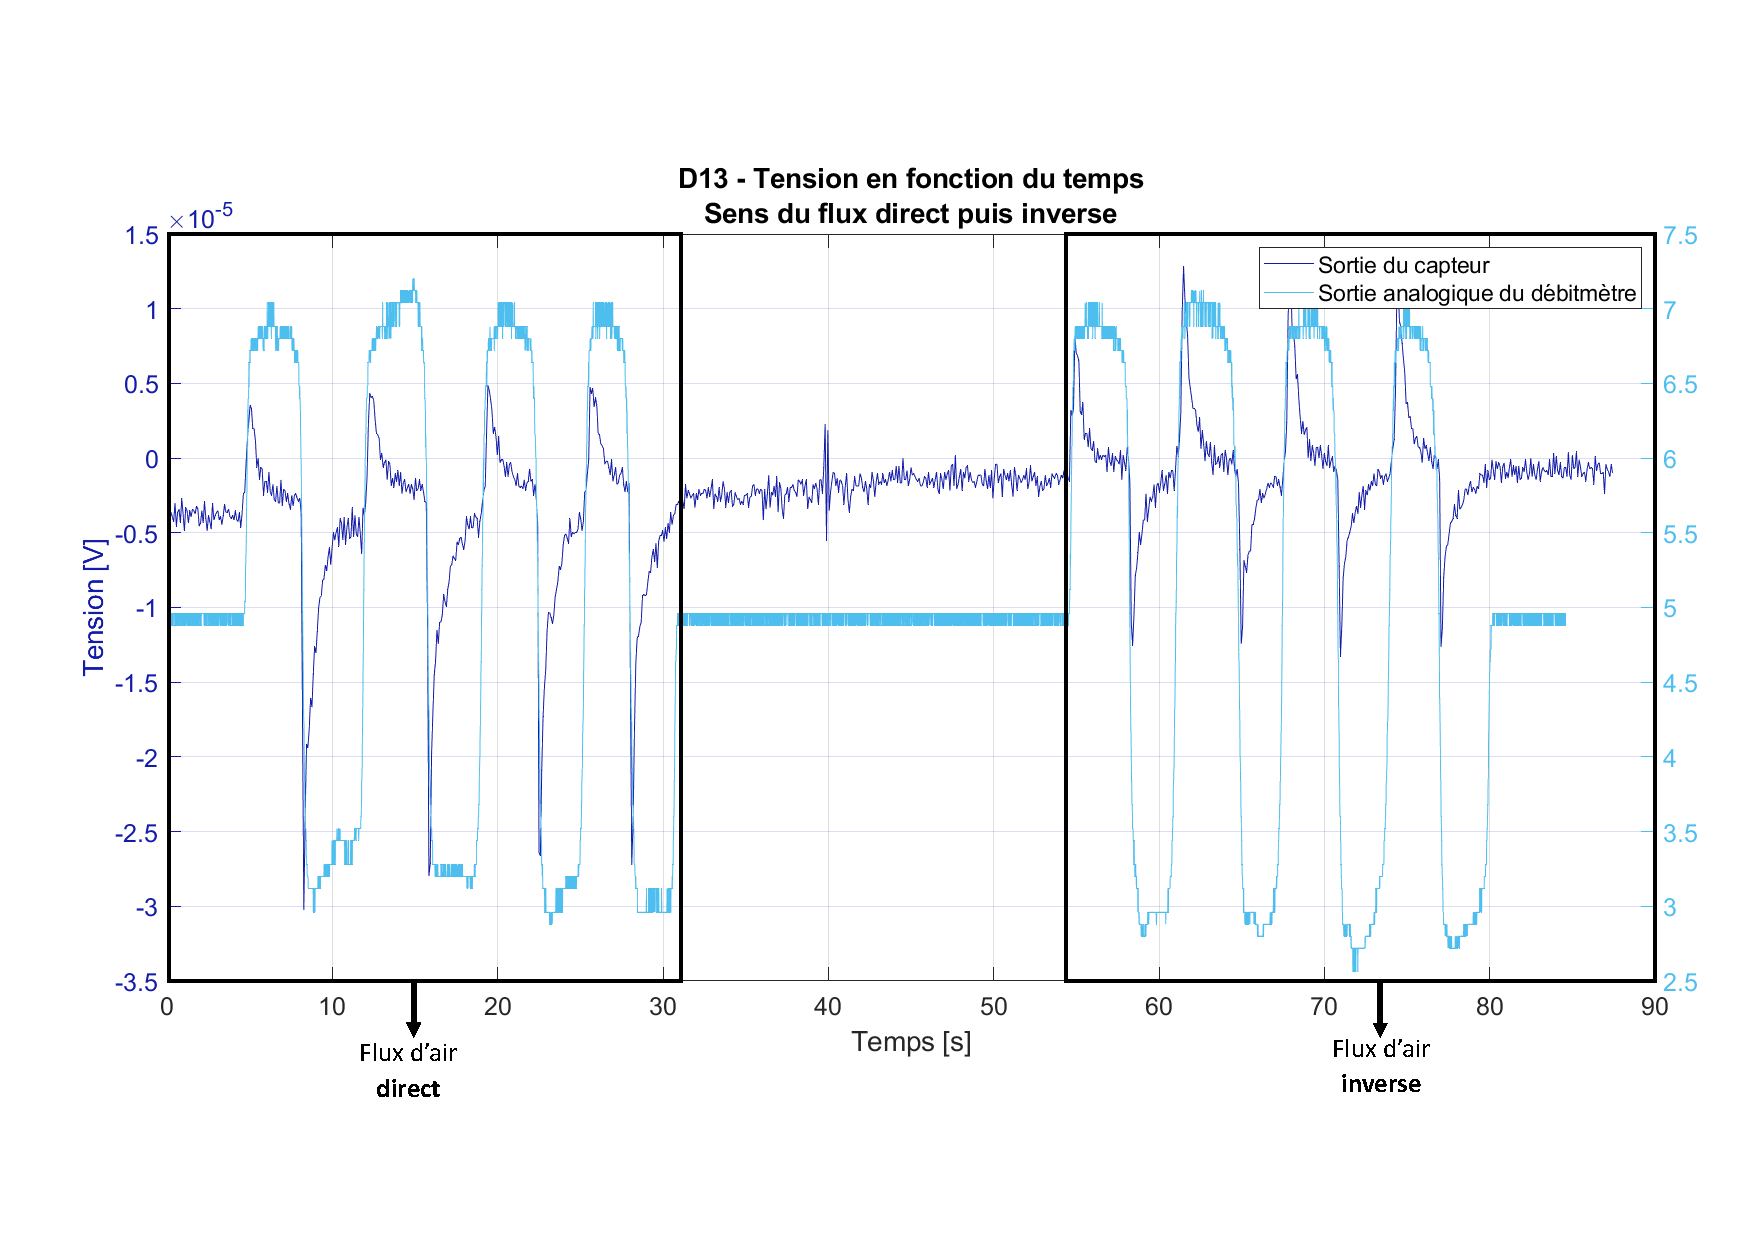
\includegraphics[scale = 0.6]{assets/figures/D13_human_breath_direct_invert_blue.pdf}
    \caption{D13 - Réponse du capteur à la respiration humaine en sens direct et inverse}
    \label{fig:D13_human_breath_direct_invert}
\end{figure}

La partie gauche du graphe de la figure \ref{fig:D13_human_breath_direct_invert}, correspond à la réponse du capteur et du débitmètre lorsque la 
respiration se fait en sens direct. La partie droite, quant à elle, montre ces deux mêmes réponses, mais lorsque la respiration se fait en sens 
inverse (cf. figure \ref{fig:direct_inverse}). 

Les mesures de la respiration humaine avec et sans corps de chauffe ont montré très peu de différences. Ainsi, le corps de chauffe a été laissé 
de côté pour le moment. 

\subsection{Mesure concernant la condensation}
Les résultats avec la respiration humaine sont bien plus nettes que ceux avec l'air comprimé. Ce phénomène peut être dû au fait que le capteur 
est sensible à l'humidité (en plus de la chaleur). De plus, étant donné que le comportement est différent lors de l'inspiration ou l'expiration, 
il était intéressant d'émettre quelques hypothèses :
\begin{itemize}
    \item L'expiration humaine est constituée d'air humide chaud qui vient donc réchauffer et humidifier le capteur
    \item L'humidité vient se déposer sur la membrane
    \item Lors de l'inspiration, il y aura un phénomène d'évaporation qui viendra changer à nouveau la température du capteur
\end{itemize}

Afin d'étudier ces hypothèses, une expérience a été effectuée en expirant seulement pendant quelques secondes (ici 5 s), puis en laissant le 
capteur reposer un certain temps. Cette manipulation permettrait d'observer si l'humidité de l'expiration s'évapore (si tel est le cas, le 
capteur devrait montrer quelque chose après l'expiration, mais avant le retour au zéro). 
\begin{comment}
\begin{figure}[H]
    \centering
    \includegraphics[scale = 0.5]{name}
    \caption{title}
    \label{fig:}
\end{figure}
\end{comment}

\section{Dépendances}
\section{Discussion}
